\documentclass[11pt]{article}

%\documentclass[11 pt]{article}
\usepackage{graphicx}
\usepackage{float}
\usepackage{tabularx,ragged2e}
\usepackage{siunitx}
\usepackage{listings}


\usepackage{rotating}
\usepackage[utf8]{inputenc}

\usepackage[square,sort,comma,numbers]{natbib}
\bibliographystyle{abbrvnat}
\setcitestyle{authoryear,open={(},close={)}} %Citation-related commands

\usepackage{setspace}\doublespacing
\usepackage[dvipsnames]{xcolor}
\usepackage{lineno}
\linenumbers
\usepackage[normalem]{ulem} 
\usepackage{multicol}
\usepackage{hyperref}
\hypersetup{
	colorlinks=false,
%	linkcolor=blue,
%	filecolor=magenta,      
%	urlcolor=cyan,
	pdftitle={Overleaf Example},
	pdfpagemode=FullScreen,
}

\addtolength{\oddsidemargin}{-2.5cm}
\addtolength{\evensidemargin}{-1.5cm}

\addtolength{\textwidth}{5.5cm}

\addtolength{\topmargin}{-.875in}
\addtolength{\textheight}{1.75in}

%\author{Pending}

\begin{document}
\begin{flushright}
%    MBE - Methods article
\end{flushright}
\begin{center}
	\begin{LARGE}
		\textbf{Pending}
	\end{LARGE}
	
	John H Tay$^1$, Sebastian Duchene$^{1, 2*}$.

$^1$Peter Doherty Institute for Infection and Immunity, Department of Microbiology and Immunology, University of Melbourne, Melbourne, Australia.

$^2$Department of Computational Biology, Institut Pasteur, Paris, France.

\end{center}
*email: sduchene@unimelb.edu.au


\begin{Large}
	\textbf{Abstract} 
\end{Large}

Pending.


\textbf{Outline}
\begin{itemize}
	\item Talk about tests of temporal signal
	\item The role of BETS
	\item pitfals of BETS: that we don't know the effect of the tree prior, all priors should be proper, impact of the clock model (because it can absorb rate variation among lineages).
	\item introduce data sets
	\item analyses of empirical data
	\subitem Use constant coalescent with the three population size priors and explain that they result in different priors on the clock rate and on the tree height. What are the implications here?
	\subitem Use the skyride and show the marginal prior on clock rate and tree height.
	\item Simulations. We should only do these for the best fitting model clock model per data set. But here, let's stick to the constant-size coalescent because it is more practical. 
	\subitem How well do they classify data sets as having temporal signal? think about error rates.
	\subitem Does the classification accuracy depend on the average logBFs for those data sets that do have temporal signal? What I mean here is that the cholera ones would naturally have stronger temporal signal than the treponema ones, so we expect different error rates. 
	\item Conclude: What is the best strategy here regarding tree prior? comment on the clock prior? where doe the regression fit in here? what about prior and posterior predictive checks?
\end{itemize}

\begin{itemize}
	\item What does the root height, tree length, and clock rate prior look in each case (coalescent with all priors, skyride)?
	\subitem How do these priors impact the phylogenetic likelihood? The point here is that if the tree prior is very wrong (i.e. it is in conflict with the likelihood) then it can mislead tests of temporal signal.
	\subitem with the relaxed clock it is useful to inspect whether the coefficient of rate variation is larger
	\item Ideally the test should assess only the sampling times
	
\end{itemize}

\textbf{\textcolor{blue}{Key points for Results section - 28 / 02 / 2024}}
\begin{itemize}
	\item The impact of the tree prior and hyperpriors on model selection. Here show the polygons and tables. Pow is particularly interesting because the exponential prior on $\Phi$ does not support temporal signal. \textbf{Result: Priors obviously impact marginal likelihoods, but sometimes also model choice}
	\item Show clock rate (ucld.mean and clock.rate) and root height distributions under each clock model and prior. \textbf{Result: Estimates of evolutionary rates and times are generally robust to the tree prior even if the marginal likelihood is not}
	\item Simulations \textbf{\textcolor{red}{Pending for now} - does the tree prior impact the accuracy to detect temporal signal?}
	\item Why does the prior on $\Phi$ impact temporal signal? Because it is linked to tree length and to the clock rate via the coalescent and the CTMC reference prior. Here show pairs plots for the root height, $\Phi$, tree length, clock rate \textbf{Result: Some parameters in the Bayesian hierarchical model are naturally correlated, the marginal prior is not obvious, but can be easily inspected}
	\item Inspecting the marginal prior is important and should be conducted prior to tests of temporal signal. For example, including monophyletic constraints, and other prior information can impact temporal signal. 
	\item Prior sensitivity is also important to assess the robustness of the estimates.
\end{itemize}

\textbf{Prior sensitivity to run (21 Feb)}
\begin{itemize}
	\item Run all three priors on $\Phi$ and check
	\subitem tree height, clock rate, tree length, pop size - and correlations
	\item Run with a set of fixed $\Phi$ values and show how the mean and variance of clock rate, tree height and tree length changes 
\end{itemize}

\textbf{new results, as of 12 Feb}
\begin{itemize}
	\item The prior on the population size seems to matter when we don't have temporal signal. It tends to lead to false positives. 
	\item A data set with temporal signal, will generally be robust to the prior. 
	\item Redefine temporal signal. It is when the data are more informative than the prior in a Bayesian context.
	\item But this is not a problem in itself. One should choose a prior that is sensible. Some data sets, like cholera will be robust to the choice of prior. They are more informative and have stronger temporal signal. 
\end{itemize}





\begin{Large}
	\textbf{Introduction}
\end{Large}

Pending


\begin{table}[H]
\caption{Proportion of simulations with temporal signal according to log Bayes factors support (log BF)}
\begin{center} 
	\label{table:logBF_pp_correspondence}
	\begin{tabular}{c|c|c|c|c}
		Prior on $\Phi$ and clock model & $log BF\ge0$ & $log BF\ge1$ & $log BF\ge3$ & $log BF\ge5$\\
		\hline
		$\Gamma(\kappa=0.001, \theta=1000)$; SC & 0.25 & 0.23 & 0.21 & 0.21 \\
		$Lnorm(\mu=1.0, \sigma=5)$; SC & 0.42 & 0.40 & 0.33 & 0.26 \\
		$Exp(\mu=1.0)$; SC & NA & NA & NA & NA \\
	\end{tabular}
\end{center}	\vspace{-0.4cm}
\end{table}


\begin{figure}[H]
	\begin{center}
		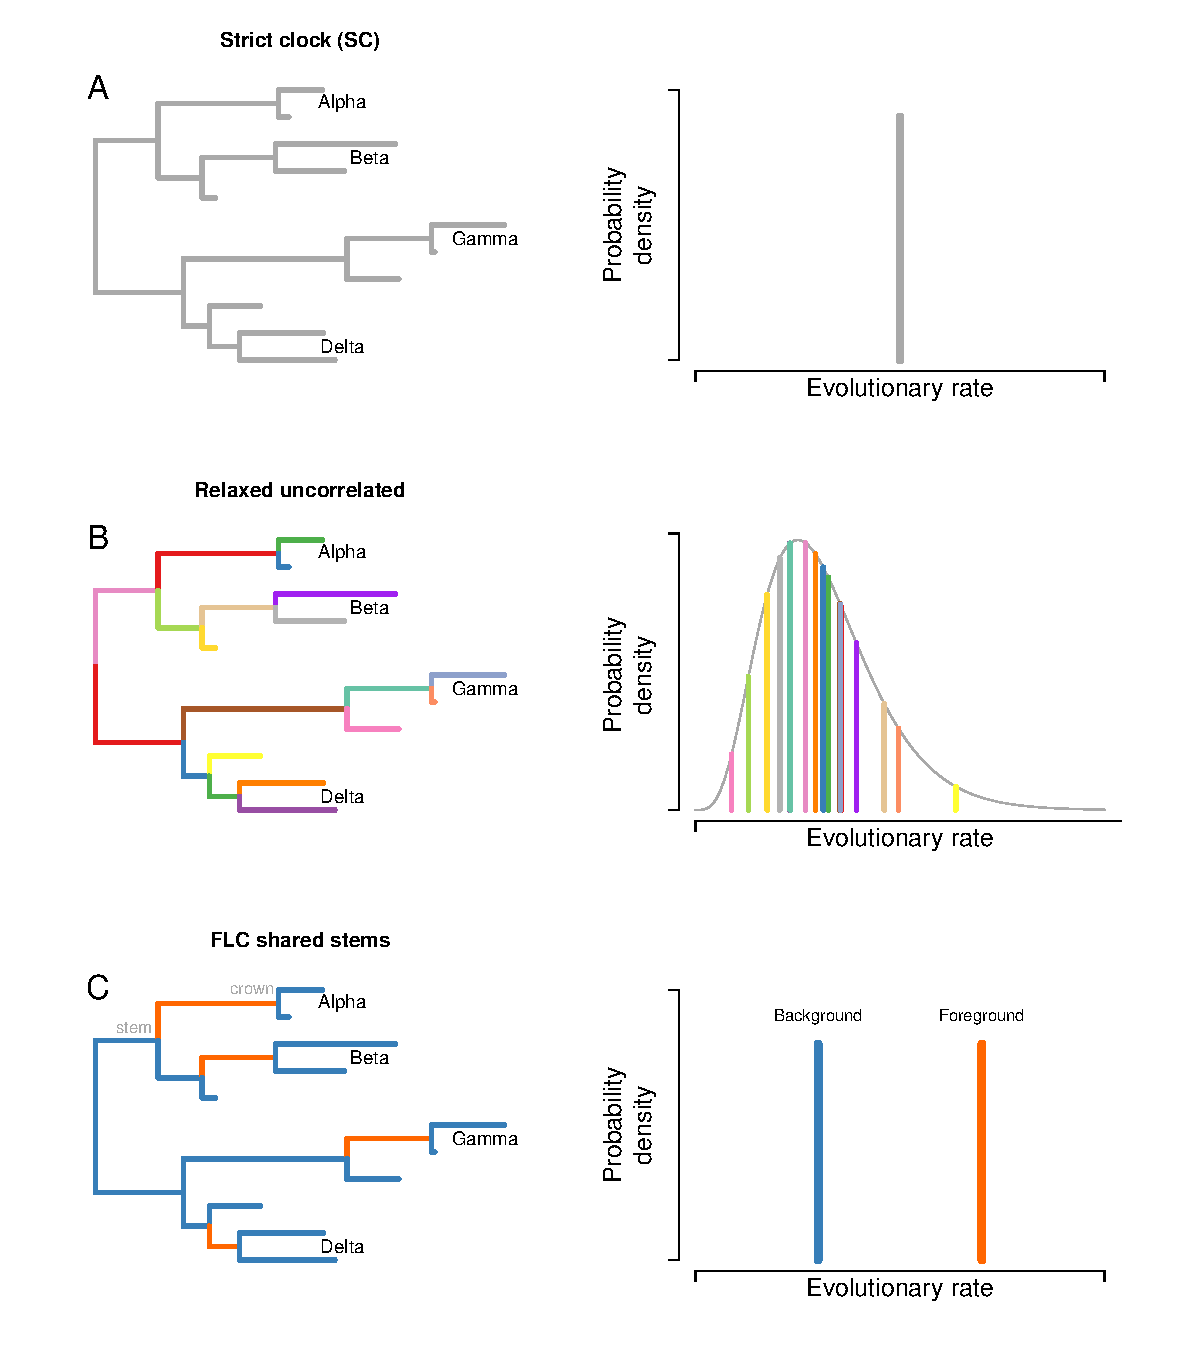
\includegraphics[width=17cm]{figures/clocks.pdf}% script: ternary_and_clock_plots.R
		\vspace{-0.5cm}
		\caption{Examples of molecular clock models. A. is a strict clock model (SC), where all branches share a single evolutionary rate. B. is an uncorrelated relaxed clock model, in which the evolutionary rates across branches are independent draws from an underlying statistical distribution, such as a lognormal or a gamma ($\Gamma$) distribution (typically abbreviated as UCLD and UCGD, respectively). Note that branches are coloured according to those drawn from the distribution on the right. C. represents a fixed local clock model, where stem branches leading up to variants of concern (VOCs; those leading to clades labelled as Alpha, Beta, Gamma and Delta, following variant names) are designated as the `foreground' and assigned a rate that differs from the `background'. In C, we have labelled the stem and crown nodes of variant Alpha, where evolutionary rate changes would have occurred.}
		\label{figure:clock_models}
	\end{center}
\end{figure}


\section{Supplementary Material}
Supplementary data are available at Molecular Biology and Evolution online.

\section{Acknowledgements}
The Authors thank two anonymous reviewers and the Editor for helpful comments in earlier versions of this manuscript. 

JHT and SD were supported by the Australian Research Council (FT220100629) and the Australian National Health and Medical Research Council (grant number 2017284). GB acknowledges support from the Internal Funds KU Leuven under grant agreement C14/18/094 and from the Research Foundation -- Flanders (`Fonds voor Wetenschappelijk Onderzoek -- Vlaanderen', G0E1420N and G098321N).
The authors acknowledge efforts by originating and submitting laboratories for the sequence data in GISAID EpiCoV on which our empirical analyses are based. This research was undertaken using the LIEF HPC-GPGPU Facility hosted at the University of Melbourne. This Facility was established with the assistance of LIEF Grant LE170100200. 

\section{Data availability}
The data underlying this article are available in GISAID at gisaid.org, and all accession numbers are provided in Supplementary Material online.

%\bibliographystyle{plain}
\bibliography{References}

\end{document}
